\documentclass{beamer}

\usepackage{minted}
\usepackage{graphicx}

\title{Test presentation}
\author{Mauri Mustonen}
\date{October 3, 2019}

\definecolor{UniBlue}{RGB}{83,121,170}
\setbeamercolor{title}{fg=UniBlue}
\setbeamercolor{frametitle}{fg=UniBlue}
%\setbeamercolor{background canvas}{bg=gray}

%\usebackgroundtemplate{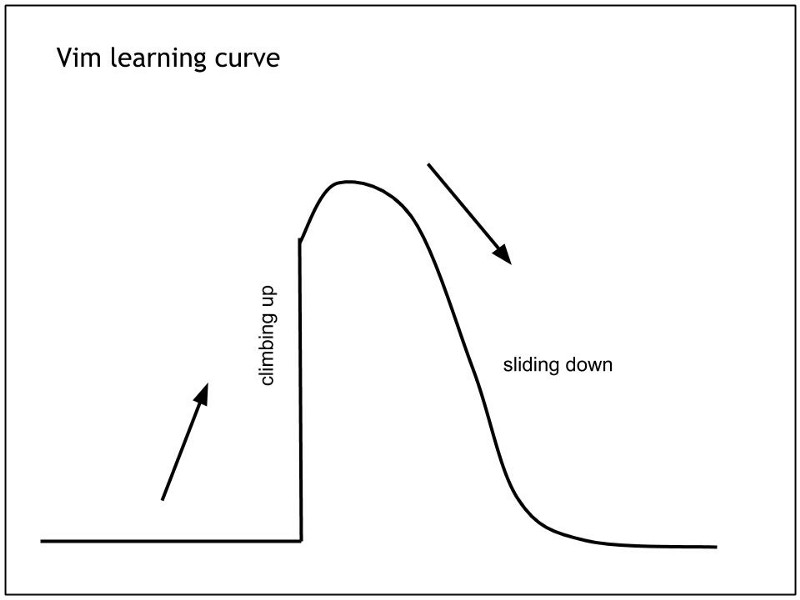
\includegraphics[width=\paperwidth,height=\paperheight]{vim.jpeg}}


\begin{document}
\maketitle

\begin{frame}[fragile]
\frametitle{Code example}
\inputminted{js}{example.js}
\end{frame}

\begin{frame}
\frametitle{Second Slide}
Contents of the second slide
\end{frame}

\end{document}

#if 0
Ideas what talk should include:
Start from basic stuff with learning wall and what vim is.
At the end Vim on different platforms (WSL for Windows).
Go through some vim features like motions, dot, registers.
Maybe show something from my .vimrc.
Go through some basic verbs and then text objects and motions on top of that. Going through these should cover pretty basic vim
usage and take some time too.
#endif
